\npara This chapter is divided into three main sections. Firstly, \textbi{\nameref{Methodology-Architecture}} proposes the architecture overview and its component in the system.
Secondly, \textbf{\nameref{Methodology-ExperimentDesign-Development}} describes tools and languages used for developing the proposed architecture.
The last part of this chapter, \textbi{\nameref{Methodology-ExperimentDesign}} elaborates how the experimental procedures will be held and how to evaluate the results.

\section{System Architecture} \label{Methodology-Architecture}

\subsection{Overall Architecture} \label{Methodology-Architecture-Overall}

\npara In this work, the reputation management system of \hyperref[Acronym-IoT]{IoT} devices is based on cloud-fog-edge architecture.
Each device in the fog layer is a node in the Ethereum Blockchain network.
In practice, the Ethereum network can be either public or private network.
However, in this work we encourage the private one because the management system is aimed to be decentralised in an \hyperref[Acronym-IoT]{IoT} system, not to be a public access for anybody.
The Smart Contracts deployed in the fog layer can store and manipulate edge devices, their services information, and geographical data of the associated regions.

\begin{figure}[hbt!]
  \centering
  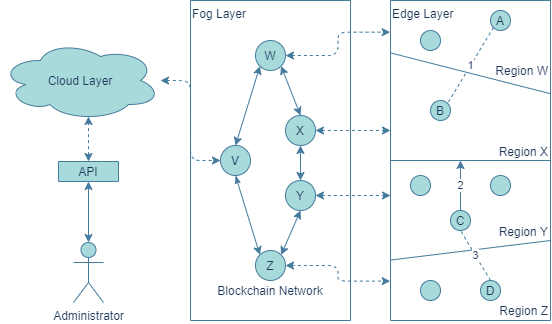
\includegraphics[width=\textwidth]{images/OverallArchitecture.png}
  \caption{Overall architecture of the proposed reputation management system}
  \label{fig:OverallArchitecture}
\end{figure}

\subsubsection*{Cloud layer}
\npara Cloud layer is generally in charge of storing and analysing data from edge sensors, as well as controlling, visualising and interacting with users.
However, in this work, because the management system is expected to be implemented in the fog layer, and the sensory data manipulation is not a protagonist in this thesis, so there will be less mentioning about this layer.
In a practical implementation of the proposed architecture, cloud layer can serve an \hyperref[Acronym-API]{API} for system administrators to control fog nodes in the layer.

\subsubsection*{Fog layer}
\npara Fog layer contains a number of devices which can be either geographically distributed or not.
These fog devices connect to each other and form an Ethereum Blockchain network \textit{to serve the Smart Contracts} for managing reputation indices and \textit{to serve the \hyperref[Acronym-API]{API}s} to interact with the contracts.
One fog device can be associated to a single or multiple regions.
However, it is not necessary because a fog device can be a Blockchain node without being associated to any regions.
For example from Figure \ref{fig:OverallArchitecture}, fog \textit{V} is not associated to any region, while fog \textit{W}, \textit{X}, \textit{Y}, \textit{Z} are associated to the region \textit{W}, \textit{X}, \textit{Y}, \textit{Z} respectively.

\subsubsection*{Edge layer}
\npara A device in this layer is equipped with sensors or actuators, and are designed to communicate with other devices in order to consume the services (dashed-line 1 from Figure \ref{fig:OverallArchitecture}).
The service consumption between devices will be based on their \textbi{trust}, which they can decide whether to trust a service provider by using the \textbi{reputation index} stored in the Smart Contracts from the fog layer.
Therefore, an edge device need to communicate with the fog layer to discover other devices in the area that provide needed services, and to query the reputation data of those providers.

\npara Furthermore, devices in the proposed system are assumed to be movable and can be displaced across the different areas.
Hence, when a device entered another area it should have a different reputation value because it is not recognised in the region.
For example, from Figure \ref{fig:OverallArchitecture}, device \textit{C} can move from region \textit{Y} to \textit{X} (arrow 2), but once it has moved, device \textit{D} which is its consumer should not anymore recognise its reputation.
And to consume the service it should establish a new connection with another device in the area that it can secondly trust.

\subsection{Scenario and Interaction Flows} \label{Methodology-Architecture-Flows}

\npara To achieve the architecture in Figure \ref{fig:OverallArchitecture} from the last section (\ref{Methodology-Architecture-Overall}).
This section elaborates the usage context of the architecture by designing interaction flows between each role in the system.
These flows will help to understand the functionalities of different components in the system, which are important for development design of programming classes and functions in the implementation section.

\npara The location-based reputation management system plays a role in the \hyperref[Acronym-IoT]{IoT} system when an end device has moved, or has requested to establish a connection with another device.
Therefore, this section divides the related interaction flows into three categories, which are 1) \textit{region management flow} which happens when there is a fog layer wants to associate itself to a geographical region in the system, 2) \textit{edge device mobility flow} which happens when an edge device has moved within the same or between different regions, and 3) \textit{reputation management flow} which happens when an edge device wants to consume a service from another device.

\begin{figure}[htb!]
  \centering
  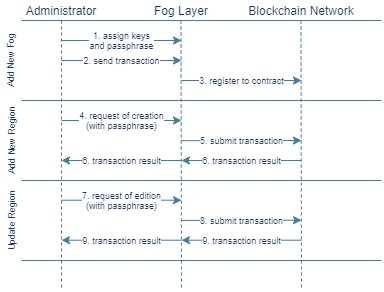
\includegraphics[width=0.8\textwidth]{images/WorkflowManageRegion.png}
  \caption{The workflow of region management in the system}
  \label{fig:WorkflowManageRegion}
\end{figure}

\npara Firstly, Figure \ref{fig:WorkflowManageRegion} shows the interaction when a fog node needs to assign or modify itself with a geographical area.
First of all, if the fog node is a new Blockchain node in the network, it needs to be assigned to an Ethereum address with a private key from the administrator (arrow 1).
After the device has been assigned to a unique Ethereum address, it can now interact with the Blockchain network.
Then, the administrator will send a contract transaction to register the node (arrow 2, 3).
After the node has been registered, it can now associate itself to a region to record that the region is in its responsibility.
The same flow happens when the node wants to update its region data.
To do so, the administrator calls a request of addition or edition to the fog node (arrow 4, 7), the node then interact with the Blockchain network to handle the request (arrow 5, 8).

\begin{figure}[htb!]
  \centering
  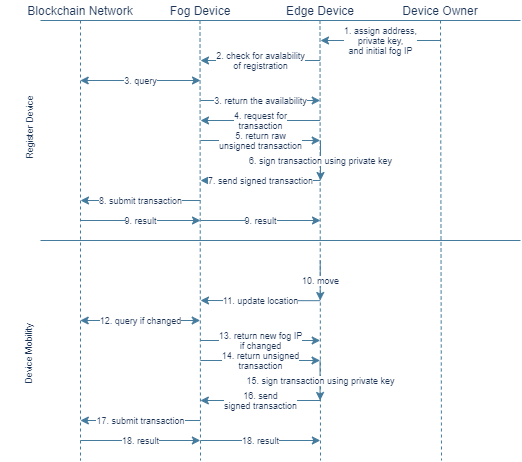
\includegraphics[width=\textwidth]{images/WorkflowMobility.png}
  \caption{The workflow of edge device mobility}
  \label{fig:WorkflowMobility}
\end{figure}

\npara Secondly, since the reputation values stored in the system are based on the device locations, it is necessary to consider the consequence when an end device has updated its location.
Figure \ref{fig:WorkflowMobility} shows the flow of the action.
As same as the fog layer, a device in the edge layer also needs its own identity in the Blockchain network so that it can interact with the Smart Contracts.
Hence, it is necessary to register a device to the Smart Contracts when it has been added to the system.
To do so, the device owner must assign a unique Ethereum address and its private key to the device (arrow 1).
Then, the device sends a contract transaction for registering.
However, due to the hardware limitations of those devices in the edge layer, it will be too big for them to store the contracts interface and be a Blockchain node.
For this reason, the interaction between the edge devices and the Smart Contracts will be done through the fog layer.
After the fog layer receives a \textit{registration request} from an edge device (arrow 4), it generates a \textit{raw unsigned transaction} and gives it back to the device (arrow 5).
The fog layer cannot sign the transaction for the edge device because it does not know the private key.
The edge device signs the transaction (arrow 6) and send the signature back to fog layer (arrow 7).
The fog layer submits the transaction to the Blockchain network (arrow 8).

\npara After the edge device has been registered, it can be referred in the Smart Contracts by using its Ethereum address.
Then, when the device has moved, it sends the updated location to the fog layer to check for the update if needed (arrow 11, Figure \ref{fig:WorkflowMobility}).
The fog layer checks with the Smart Contract whether it is necessary to update the device location data (arrow 12), in case of yes, it returns an unsigned transaction back to the device (arrow 14).
The device signs the transaction and return the signature to the fog layer (arrow 15, 16).

\begin{figure}[htb!]
  \centering
  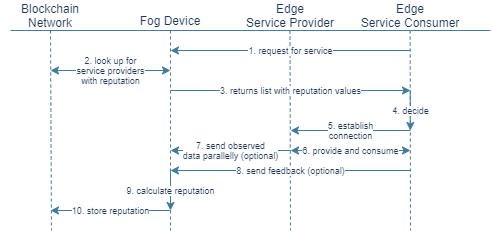
\includegraphics[width=\textwidth]{images/WorkflowReputation.png}
  \caption{The workflow of reputation query and generation}
  \label{fig:WorkflowReputation}
\end{figure}

\npara The last event is when a device wants to consume a service.
Figure \ref{fig:WorkflowReputation} shows the flow of this interaction.
The consumer requests for a service to the fog layer.
The fog node handles it by looking up for the results in the Smart Contracts (arrow 1, 2).
Then, it returns a list of candidate service providers and their reputation values in the area back to the consumer (arrow 3).
The consumer considers from this list and establish a new connection with the provider which it trusts the most (arrow 4, 5).
While the connection is ongoing (arrow 6), the service provider can parallelly sends the data to the fog device (arrow 7), which can later use these data to calculate the service quality as a factor of generating a new reputation index.
After the connection is finished, the consumer can send its feedback regarding the service to the fog node (arrow 8).
The fog layer finally have both sensory data from the provider and a feedback from the consumer, it then can use these information to calculate a new reputation index of the service provider (arrow 9) and update the value in the Smart Contracts (arrow 10).

\subsection{Fog Layer} \label{Methodology-Architecture-RMS-Fog}

\npara In the fog layer, there are two sub-components: \textbi{Ethereum Blockchain Network} which stores Smart Contracts of managing device information and the reputation data.
The second sub-component is \textbi{Fog \hyperref[Acronym-API]{API}} which is an \hyperref[Acronym-HTTP]{HTTP} interface for communication with the administrator users and edge devices.

\subsubsection{Ethereum Smart Contracts}

\begin{figure}[htb!]
  \centering
  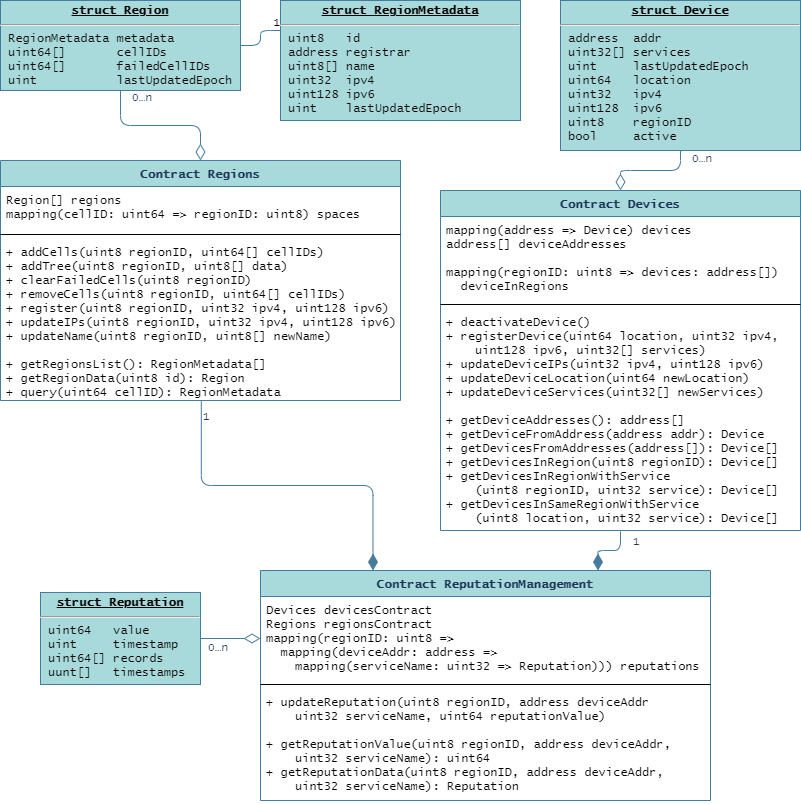
\includegraphics[width=\textwidth]{images/Contracts.png}
  \caption{Class diagram of the Smart Contracts}
  \label{fig:ContractsDiagram}
\end{figure}

A Smart Contract in the Ethereum Blockchain network can be written in \textit{Solidity} programming language.
The syntax of Solidity allows an object-oriented way of programming.
Hence, the structure of a Smart Contract can be described using a diagram similar to programming in other \hyperref[Acronym-OOP]{OOP} languages such as C\verb|#| or Java.
Nevertheless, the computation is slightly different comparing to a traditional programming language as there are some points needed to concern when doing Smart Contracts programming, such as:

\begin{itemize}
  \item Methods in Solidity can return more than one values.
  \item Decimal number: float or double, is not fully supported in Solidity \citep{SolidityTypes}, so integer or big integer is more encouraged.
  \item Similarly, strings are also not fully supported in Solidity.
  For this reason, manipulating and storing textual data should be done in binary level.
  \item When sending a contract method transaction, the Smart Contract always knows who is the transaction sender.
  Therefore, it is not necessary to define a caller in the method parameters.
\end{itemize}

\npara Figure \ref{fig:ContractsDiagram} shows the Smart Contract diagram of the proposed architecture.
There are three contracts in this proposed architecture:
  \textbi{Regions Contract} which manages the regions and their geospatial areas,
  \textbi{Devices Contract} which manages devices in the system and their service information,
  and finally \textbi{Reputation Management Contract} which enables updating and querying the reputation value in different regions.
In practice, each contract will have only one instance.
The regions and devices contract can be initiated and have an instance by their own.
In contradiction, the reputation management contract is dependent on the regions and devices contract in order to be functional.

\subsubsection{Fog API}

\npara Fog \hyperref[Acronym-API]{API} is another component inside a fog device which connects users to the Smart Contracts.
A user of this \hyperref[Acronym-API]{API} can be either the administrator who manages the system, or the edge devices that communicate for discovering service providers and their reputation values in an area.
The \hyperref[Acronym-API]{API} serves on \hyperref[Acronym-HTTP]{HTTP} protocol accepting the requests and returning responses in a \hyperref[Acronym-JSON]{JSON} format.
It communicates with the Ethereum client to serve the requests.
It also performs a preliminary condition checking before calling the Smart Contract to avoid an unexpected failure transaction.

\begin{figure}[ht]
  \centering
  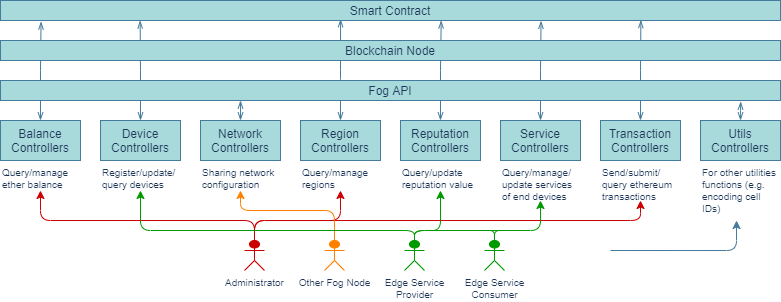
\includegraphics[width=\textwidth]{images/FogAPIs.png}
  \caption{Controllers and interaction diagram of Fog \hyperref[Acronym-API]{API}}
  \label{fig:FogAPIs}
\end{figure}

\npara The interaction interface of the Fog \hyperref[Acronym-API]{API} is divided into a number of different controllers which are listed in Figure \ref{fig:FogAPIs}.
Each controller serves a different propose and interact with different users in the system.
Most of the controllers require a connection to the Blockchain in order to query or submit a Smart Contract transaction, while some controllers are designed for the other facility and calculation proposes so they do not require any communication with the Ethereum client.

\subsection{Edge Layer} \label{Methdology-Architecture-RMS-Edge}

\npara The communication of edge devices in this work are also based on \hyperref[Acronym-API]{API} over \hyperref[Acronym-HTTP]{HTTP} protocol.
The device exposes its \hyperref[Acronym-IP]{IP} address and serves its \hyperref[Acronym-API]{API} in a defined port, so that a service consumer can communicate to consume the service.
Despite the fact that \hyperref[Acronym-HTTP]{HTTP} is used in the development of this work, it is not obligatory that another implementation adopting the architecture has to use the same communication technology.
The system architecture allows another technology as well, depending on their requirements and hardware specifications, \hyperref[Acronym-MQTT]{MQTT} for instance.
Nevertheless, to accomplish the proposed interaction flow, a device in this layer should be able to perform the calculation of signing a transaction using \textit{Elliptic Curve Digital Signature Algorithm (\hyperref[Acronym-ECDSA]{ECDSA})} which is a digital signature algorithm used in the Ethereum network.

\subsection{Geographical Data in the Smart Contract} \label{Methodology-SpatialSmartContract}

\begin{figure}[htb!]
    \centering
    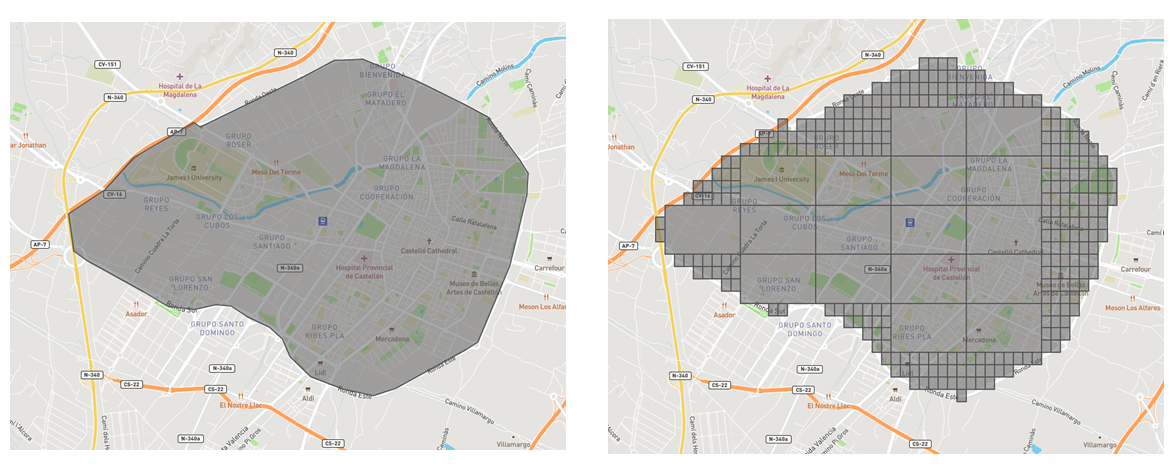
\includegraphics[width=\textwidth]{images/PolygonAndGeohashes.png}
    \caption{Example of a polygon covered by geocoded cells}
    \label{fig:PolygonAndGeohashes}
\end{figure}

\npara As described in the previous sections (\ref{Background-SpatialIndexing}, \ref{Methodology-Architecture-RMS-Fog}), this thesis decided to use geocoding techniques to store the geographical areas (polygons) of the associated regions in the Smart Contracts to manage the reputation and perform a spatial query.
Figure \ref{fig:PolygonAndGeohashes} shows an example of the geocoded regions.
The left image shows the original polygon of the region.
The data stored in the Smart Contract will be a set of geocoded cells shown in the right image.
Because of that the binary representation of the adopted geocoding techniques is hierarchical, it can merge the group of cells which fulfil the lower level into one cell in the upper level.
This behaviour can be observed from the right image of Figure \ref{fig:PolygonAndGeohashes}.
The cells in the centre of the region are merged into one bigger cell.

\begin{figure}[htb!]
  \centering
  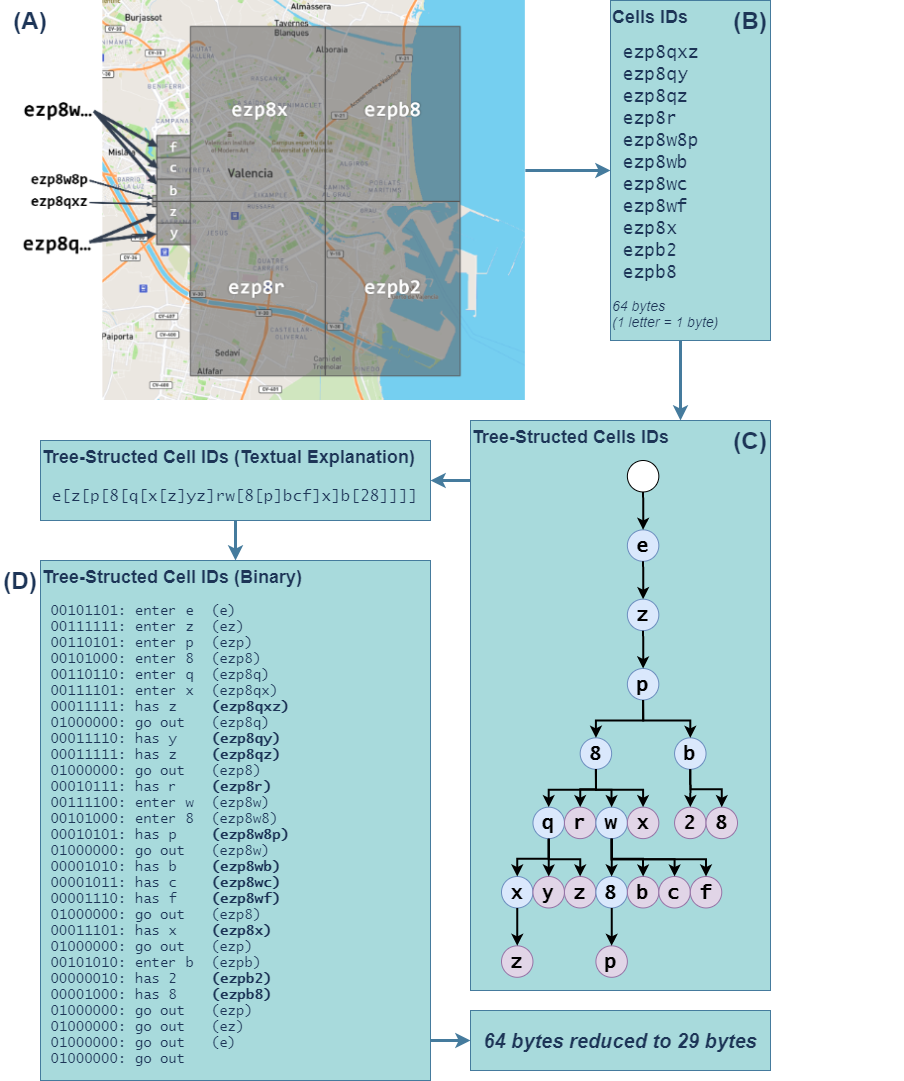
\includegraphics[width=\textwidth]{images/GeocodingCompression.png}
  \caption{An example of the proposed geocoded cells compression technique}
  \label{fig:GeocodingCompression}
\end{figure}

\npara Figure \ref{fig:GeocodingCompression} shows another example of geocoding a region.
Part \textit{(A)} of the figure shows the geocoded region cells and their identification using Geohash.
There are 11 cells from 3 different levels in this example.
Part \textit{(B)} of the figure shows the cell identification list of the region.
When a letter consumes 1 byte in the memory, this list of Geohash cells will consume at least 64 bytes of data, excluding cell separation such as a new-line character.
From this list it can be observed that there are redundancy of the data, especially the prefix of those cells.
Therefore, this work will also propose a compression technique of geocoded cells based on tree structure.
Part \textit{(C)} of Figure \ref{fig:GeocodingCompression} shows the tree-based structure of this geocoded region.
The nodes in blue colour represent the cells that have children, while the nodes in purple colour represent the final level that will be included in the region data.
This tree structure can be encoded into binary representation shown in part \textit{(D)} of the figure.
Because a Geohash cell uses \hyperref[Appendix-Base32]{\textit{base32}} representation, which requires only 5 bits to store one level, storing it in one byte will have 3 bits remained unused.
Therefore, these 3 bits can store an additional information to indicate that the node cell has children or not.
The result from binary encoding this tree requires only 29 bytes to store the data, which is less than a half of the original data that requires 64 bytes.

\npara In the same way, an S2 cell list can also be compressed by the same algorithm.
However, an S2 cell uses 2 bits for one level, storing one level of 2-bit in one byte is not sufficient.
Therefore, the S2 cell will be grouped by 6 bits before being structured to be a tree, the spare 2 bits are used for the level open or close marking like Geohash.
A 6-bit in this S2 cell can be represented by \hyperref[Appendix-Base32]{\textit{base64}} representation.

The description of compressed data is explained in the appendix (\textit{\nameref{Appendix-GeocodingCompress}}).

%%

\section{Implementation and Development} \label{Methodology-ExperimentDesign-Development}

\npara The proposed architecture is an abstract structure and can be implemented using any programming languages and tools.
However, this section will explain the tools used for developing the proof of the architecture in this thesis.

\subsection{Fog Layer}
\npara The Ethereum network will be deployed using \textbi{Go Ethereum (Geth)}\footnote{\url{https://geth.ethereum.org/}}, which is an open-sourced implementation of the Ethereum Blockchain network using Go language.

\npara The fog \hyperref[Acronym-API]{API} will be developed by \textbi{JavaScript} language run in \textbi{NodeJS}\footnote{\url{https://nodejs.org/}} engine.
The \hyperref[Acronym-API]{API} serves requests on \hyperref[Acronym-HTTP]{HTTP} protocol using \textbi{Express}\footnote{\url{https://expressjs.com/}} library, which is available on \hyperref[Acronym-NPM]{NPM}.
The reason for using JavaScript as the programming language is because of that it can communicate with Geth client using \textbi{web3.js}\footnote{\url{https://web3js.readthedocs.io/en/}} library.
The library also allows the interaction with a Smart Contract to be done in a simpler way through \textit{Application Binary Interface (\hyperref[Acronym-ABI]{ABI})} of the contract.
Additionally, while developing the Smart Contracts, it will use \textbi{Truffle}\footnote{\url{https://www.trufflesuite.com/truffle}} which is a programming suite designed for Smart Contract development.
Truffle contains multiple tools that allow to compile, test, and deploy the developed contracts written in Solidity into the Ethereum network.

\subsection{Edge Layer}
\npara The edge devices in this work are influenced by available hardware provided by the university laboratory, which is \textbf{Particle Development Board}\footnote{\url{https://www.particle.io/}}.
The device has similar specification as \textit{Arduino}, but the Particle board allows the possibility of compiling and flashing the programme to the board using its cloud service.
So that the board does not have to be physically connected to the computer, but it needs an internet connection instead.
The programming for the device will be written in \textbi{C++} language.
As described in the section \ref{Methdology-Architecture-RMS-Edge}, the communication between edge devices will be done by \hyperref[Acronym-API]{API} on \hyperref[Acronym-HTTP]{HTTP} protocol.
Hence, the library that serves this propose is \textbi{ParticleRdWebServer}\footnote{\url{https://github.com/robdobsn/ParticleRdWebServer/}} by \textit{robdobsn}.
Lastly, the board needs to be able to sign the transactions using \hyperref[Acronym-ECDSA]{ECDSA} so it will use \textbf{micro-ecc}\footnote{\url{https://github.com/kmackay/micro-ecc}} library provided by \textit{kmackay} to do so.

%%

\section{Experiment Design} \label{Methodology-ExperimentDesign}

\npara This section describes the experiments designs and procedures, as well as their evaluation.
It is divided into three subsections, which are
  \textbi{\ref{Methodology-ExperimentDesign-TechniquesComparison} \nameref{Methodology-ExperimentDesign-TechniquesComparison}} defines the procedures and criteria of comparison between the two geocoding techniques and the proposed compressing algorithms (\ref{Methodology-SpatialSmartContract}),
  \textbi{\ref{Methodology-ExperimentDesign-Simulation} \nameref{Methodology-ExperimentDesign-Simulation}} which describes the simulation of the proposed architecture to test the different aspects,
  lastly \textbi{\ref{Methodology-ExperimentDesign-Deployment} \nameref{Methodology-ExperimentDesign-Deployment}} describes the implementation methodologies and the test case scenario.

\subsection{Experiment: Geocoding Techniques Comparison} \label{Methodology-ExperimentDesign-TechniquesComparison}

\npara To answer \hyperref[ResearchQuestion-Geocoding]{\textit{the research question \ref{ResearchQuestion-Geocoding}}}, this experiment is designed to compare between Geohash and S2 geocoding techniques.
Although \hyperref[RelatedWorks]{\textit{the related works}} have already indicated that S2 performs better in many aspects, there are still more aspects to compare for the compatibility in the proposed algorithm.

\npara The comparison will be performed by:
\begin{enumerate}
  \item Covering or fitting a Geo\hyperref[Acronym-JSON]{JSON} polygon into a list of geocoded cells \textit{(using data of the administrative regions in Spain)}
  \item Compressing geocoded cells using the proposed algorithm
\end{enumerate}
In each step, it will compare the result by their output size and calculation time

\subsection{Experiment: Contract Simulation} \label{Methodology-ExperimentDesign-Simulation}

\npara The second part of the experiments is to develop the Smart Contracts of the proposed architecture and test their performance.
This experiment is designed to prove the architecture functionality, which will answer \hyperref[ResearchQuestion-DecentralisedFog]{\textit{the research question \ref{ResearchQuestion-DecentralisedFog}}}.
It is also designed to test the manipulation of spatial data in the Smart Contracts, which was mentioned in \hyperref[ResearchQuestion-SpatialBlockchain]{\textit{the research question \ref{ResearchQuestion-SpatialBlockchain}}}.
Lastly, it will be conducted twice in the Smart Contracts based on both Geohash and S2 to compare and answer \hyperref[ResearchQuestion-Geocoding]{\textit{the research question \ref{ResearchQuestion-Geocoding}}} as well.
The procedure in this experiment is to measure the following:
\begin{enumerate}
  \item Gas used to deploy the developed contracts into an Ethereum network
  \item Input size and time spent for adding regions using Geohash and S2, either cell array or the compressed tree
  \item Time spent to query for a cell in the Smart Contract based on Geohash and S2
  \item Time spent to mine a block in an Ethereum blockchain using a personal computer and a fog device (Raspberry Pi)
\end{enumerate}

\subsection{Experiment: Deployment and Scenario} \label{Methodology-ExperimentDesign-Deployment}

\npara The last experiment is to answer \hyperref[ResearchQuestion-DecentralisedFog]{\textit{the research question \ref{ResearchQuestion-DecentralisedFog}}} by proving that the proposed architecture works in the \hyperref[Acronym-IoT]{IoT} devices by deploying the programme into both fog and edge devices.
The fog devices used in this experiment are \textit{Raspberry Pi}, while the edge devices are \textit{Particle Development Board}.
The experiment will set up the developed programme into the devices and use the described workflow to test the communication between them.
The expectation in this experiment is to confirm that:
\begin{enumerate}
  \item A fog node is able to serve as an Ethereum node
  \item A service consumer is able to discover the available providers and their reputation data, as well as provide a feedback after the consumption
  \item A service provider is able to provide the service and able to sign the transaction
\end{enumerate}
